\section{Outils de travail}

\subsection{Gestionnaire de version}
Les premiers échanges que nous avons eu après l'attribution du sujet se sont concentrés sur le choix du gestionnaire de version que nous allions utiliser au cours du projet. Ce gestionnaire de version permet en autre de :
\begin{itemize}
\item Partager le code source de l'application.
\item Gérer des conflits lors de la modification simultané d'un fichier.
\item Maintenir l'ensemble des versions d'un ou plusieurs fichiers.\\
\end{itemize}

Etant majoritairement habitué à utiliser Git, c'est vers un dépot \textbf{Github} que nous nous sommes tourné.

\subsection{Répartition des t\^aches}
Au cours de leurs formations antérieures, certain membres du projet ont eu l'habitude d'utiliser l'outil de gestion de projet \textbf{Trello}. C'est pourquoi nous avons utiliser cet outil pour répartir les t\^aches.\\

\textbf{Trello} permet de découper en <Tickets> les différentes t\^aches à réaliser. Ces tickets peuvent \^etres déplacés par les membres du projets dans différentes catégories :
\begin{itemize}
\item \textbf{TODO} - les t\^aches qu'il restent à faire. 
\item \textbf{DOING} - les \^aches en cours de develloppement.
\item \textbf{DONE} - les t\^aches qui sont terminées.
\item \textbf{TESTS} - les t\^aches qui sont validées et testées.\\
\end{itemize}
Chaque membre choisi un ticket dans la partie TODO et le déplace dans DOING puis lorsqu'il a terminé dans DONE et pour finir dans TEST.

\subsection{Communication}
Les outils de communication ont évolué au cours du projet. Nous avons tout d'abord utilisé naturellement la messagerie instantanée que propose \textbf{Facebook}. Cette messagerie simple et permet de partager des images ainsi que des documents.

Cependant nous souhaitions pouvoir discuter à l'oral ce que ne permet pas facilement la messagerie de Facebook. C'est pour cette raison que nous avons migré sur le logiciel \textbf{Discord} qui permet, en plus de la messagerie et de l'échange de documents, de discuter à l'oral ce qui a grandement facilité notre communication.
De plus, nous avons installé un BOT sur le Discord, lié a GitHub, qui écrit un message lors d'une modification du dép\^ot git (figure \ref{bot_discord}).

\begin{figure}[!h]
\centering
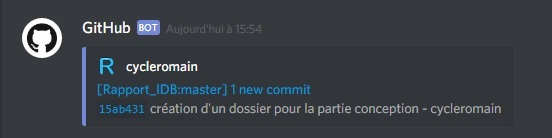
\includegraphics[width=10cm]{./images/activite/bot_discord.jpg}
\caption{Message du BOT Discord lié à GitHub}
\label{bot_discord}
\end{figure}

\subsection{Partage de documents}
Tout au long du projet, nous avons produits différents documents qu'il nous a fallu stocker dans un endroit facile d'accès pour tous. Nous avons donc créé un dossier sur un \textbf{Google Drive} et l'avons partagé aux membres du groupe. Ce Drive nous a permis d'échanger et stocker des diagrammes, des pdf, des documents texte, des maquettes pour les \glspl{ihm}* ainsi que d'autres fichiers que nous voulions conserver.

\section{Planification}